\section{Theorie}
	
	Im Folgenden sollen zunächst die theoretischen Grundlagen für die nachfolgenden experimentellen Untersuchungen erörtert werden. Ausgehend von allgemeinen Grundlagen, wie Kernniveaus, $\gamma$-Zerfall und die Hyperfeinstruktur, wird dann der hier untersuchte Mößbauer-Effekt erklärt. Die vorgestellte Theorie basiert auf Schatz und Weidinger.\cite{schatz}
	
	\subsection{Kernniveaus und Übergänge}
	
	\subsubsection{Emission und Absorption von $\gamma$-Quanten}
	
	Analog zum Schalenmodell für die Elektronen in der Atomhülle, lässt sich auch für den Atomkern ein solches definieren. Auch hier treten gegenüber dem Grundzustand angeregte Zustände auf, die durch verschiedene Quantenzahlen (Hauptquantenzahl, Kernspin, ...) gekennzeichnet sind.
	
	Nach $\alpha$- und $\beta$-Zerfällen liegen die die Kerne oft in einem angeregten Zustand vor. Die \glqq Abregung\grqq\ geschieht meist über die Aussendung von $\gamma$-Quanten, also hoch-energetischen Photonen. Im Gegensatz zu den elektromagnetischen Übergängen in der Atomhülle, wo fast nur Dipolstrahlung auftritt, sind bei den Übergängen im Kern höhere Multipole (Quadrupol, Oktupol, ...) nicht zu vernachlässigen. 
	
	\noindent Statt der Emission von Photonen kann die Energie auch an ein Elektron in der Hülle des Atoms abgegeben werden, welches dadurch aus dem Atom herausgeschlagen wird (Konversionselektronen). Im Gegensatz zur $\beta$-Strahlung entstammen diese jedoch nicht dem Kern selbst und besitzen außerdem ein diskretes Energiespektrum. Bei sehr hohen Energien ist zudem die Bildung und Emission eines Elektron-Positron-Paares im Kern möglich (Paarkonversion).
	
	Umgekehrt kann ein Atomkern, wenn ein Photon mit genau der zu einem Übergang zwischen zwei Kernniveaus passenden Energie auf diesen trifft, unter Absorption des Photons wiederum in einen angeregten Zustand übergehen. Unter der Annahme, dass die Energieniveaus des Atomkerns diskret sind, würde man zunächst vermuten, dass ein Photon, welches von einem Atomkern emittiert wurde, ohne Probleme von einem anderen Atomkern des gleichen Typs absorbiert werden kann. Dabei treten jedoch einige Hindernisse auf, welche im folgenden Abschnitt diskutiert werden sollen.
	
	\subsubsection{Natürliche Linienbreite und Rückstoßeffekte}
	
	Verschiedene Faktoren sorgen dafür, dass die Linie eines Kernniveaus im Energiespektrum verbreitert wird. Als erstes ist die natürliche Linienbreite zu nennen, die aus der quantenmechanisch begründeten Unschärfe resultiert. Die Halbwertsbreite der hier betrachteten $14,4\,$keV-Linie von $^{57}$Fe mit einer Lebensdauer von $\tau_N=1,41\cdot 10^{-7}\,$s berechnet sich zu $\Gamma = \hbar/\tau_N=4,7\cdot10^{-9}\,$eV. Diese vorgegebene Breite ist prinzipieller Natur und durch keinerlei Verfahren beeinflussbar.
	
	Man betrachte nun einen frei beweglichen Atomkern, z.\,B. in einem idealen Gas. Er besitze den Impuls $\vec{p}=M\vec{v}$ (nach klassischer Vorstellung) und sei in einem angeregten Zustand der Energie $E_a$. Unter Aussendung eines Photons mit der Energie $\hbar \omega$ und dem Impuls $\hbar \vec{k}$ gehe der Kern in den Grundzustand mit der Energie $E_g = E_a -\hbar\omega_0$ über. Man erhält:
	\begin{align}
		\hbar \omega = \left( E_a + \frac{\vec{p}^2}{2M}\right)  - \left( E_g  + \frac{\left( \vec{p}-\hbar \vec{k}\right) ^2}{2M}\right) = \hbar\omega_0 + \hbar\left( \vec{k} \cdot \vec{v}\right) -\frac{\hbar^2k^2}{2M}
	\end{align}
	Die Energie des Photons ist also einerseits um einen konstanten Rückstoßterm $\frac{\hbar^2k^2}{2M}$ zu geringeren Energien verschoben. Dieser Term ist typischerweise von der Größenordnung $10^{-3}\,$eV. Die Geschwindigkeiten der Atome in einem idealen Gas sind statistisch um $v=0$ verteilt. Der Doppler-Effekt-Term $\hbar\left( \vec{k} \cdot \vec{v}\right)$ sorgt dementsprechend für eine Verbreiterung der Linie des Übergangs in der Größenordnung $10^{-2}\,$eV. 
	
	Wird ein Photon hingegen absorbiert, kehren sich die Vorzeichen der oben genannten Terme um, d.\,h. die Linie ist zu höheren Energien hin verschoben. Die Stärke dieser Rückstoßeffekte übersteigt die der natürlichen Linienverbreiterung um mehrere Größenordnungen.
	
	\subsubsection{Hyperfeinstruktur}
	
	Die Hyperfeinstruktur beschreibt den Einfluss von elektrischen und magnetischen Feldern auf die Kernniveaus. Als erstes ist das magnetische Kerndipolmoment zu nennen, welches zu einer Aufspaltung der Niveaus führt. Sei $I$ der Kernspin und $M$ die zugehörige magnetische Quantenzahl (Komponente in $z$-Richtung), dann ist die Energieverschiebung des Niveaus $E_\text{magn.}$ gegeben durch:
	\begin{align}
		E_\text{magn.}=-g(I)\mu_\text{N}B_z M
	\end{align}
	Dabei ist $g(I)$ der Land\'{e}-Faktor, $\mu_\text{N}=\frac{e\hbar}{2m_p}\approx 5,05\cdot 10^{-27}\,$m$^2$A das Kernmagneton und $B_z$ die $z$-Komponente des Magnetfeldes. Die Niveaus spalten also äquidistant auf. Das magnetische Moment eines Niveaus ist gegeben durch:
	\begin{align}
		\mu = g(I)\mu_\text{N}I
	\end{align}
	Als nächstes wird das elektrische Kernquadrupolmoment $Q$ betrachtet. Es gibt die Abweichung der Ladungsverteilung im Kern von einer Kugelform an, dementsprechend ist es für den Fall einer kugelsymmetrischen Ladungsverteilung null. Für Niveaus mit Kernspin $I<1$ ist es außerdem auch immer null. 
	
	Auch das elektrische Kernquadrupolmoment sorgt für eine Aufspaltung der Niveaus analog zum magnetischen Dipolmoment, hängt jedoch nur vom Betrag der magnetischen Quantenzahl $M$ ab. Die Energieverschiebung eines Niveaus, das der Quadrupolwechselwirkung unterliegt, berechnet sich zu:
	\begin{align}
		E_Q(M)=\frac{eQV_{zz}}{4I(2I-1)}\left( 3M^2 - I(I+1)\right) 
	\end{align}
	Hierbei ist $V_{zz}$ der elektrische Feldgradient in $z$-Richtung.
	
	Neben der Quadrupolwechselwirkung gibt es auch noch eine Monopolwechselwirkung, welche einen Einfluss auf die Kernniveaus hat. Diese führt später auf die sogenannte Isomerieverschiebung. Ist $\left\langle r^2\right\rangle $ der Erwartungswert des quadratischen Kernradius und $\left| \psi(0)\right|^2$ die Elektronendichte am Kernort, ergibt sich die Energieverschiebung:
	\begin{align}
		E_C = \frac{Ze^2}{6\epsilon_0}\left| \psi(0)\right|^2\left\langle r^2\right\rangle \label{eq:monopol}
	\end{align}
	
	\subsection{Der Mößbauer-Effekt}
	Die im letzten Abschnitt diskutierten Effekte der Hyperfeinstruktur waren lange Zeit aufgrund ihrer geringen Größenordnung gegenüber dem Rückstoßeffekt nicht messbar. Rudolf Mößbauer beobachtete den nach ihm benannten Effekt, durch den Kerne Photonen rückstoßfrei emittieren und absorbieren können. 
	
	Dazu baut man den jeweiligen Kern in ein Kristallgitter ein. Innerhalb dessen kann ein Kern höchstens zu Schwingungen angeregt werden. Diese Schwingungen liegen quantisiert in Form von Phononen vor. Werden bei der Emission bzw. Absorption eines Photons keine Phononen erzeugt oder vernichtet, so wird der Impuls an den gesamten Kristall übertragen. Aufgrund der großen Masse des Kristalls wird dabei kaum Energie übertragen. Die Wahrscheinlichkeit für eine solche rückstoßfreie Emission bzw. Absorption wird durch den sogenannten Debye-Waller-Faktor angegeben. 
	
	\subsubsection{Debye-Waller-Faktor}
	
	Der Debye-Waller-Faktor $f$ gibt das Verhältnis der unverschobenen und unverbreiterten $\gamma$-Emissionen/Absorptionen zu allen $\gamma$-Emissionen/Absorptionen an. Er lässt sich innerhalb einfacher Modelle wie dem Einstein- oder dem Debye-Modell gut berechnen. Im Debye-Modell erhält man:
	\begin{align}
		f=\exp\left[ -\frac{\hbar^2k^2}{2M}\cdot\frac{3}{2k_B\Theta_D}\left( 1+\frac{2\pi^2}{3}\cdot\left( \frac{T}{\Theta_D}\right)^2\, \right) \right]
	\end{align}
	Er wird demnach bei kleineren Temperaturen $T$ größer. Da eine Kühlung sehr langwierig und energieaufwändig ist, wird hier davon abgesehen. Die anderen auftauchenden Größen, wie der Impuls des $\gamma$-Quants $\hbar k$, die Masse des Emitter-/Absorberatoms $M$, die Boltzmann-Konstante $k_B$ und die Debye-Temperatur $\Theta_D$, sind allesamt vom Material bzw. Niveau abhängig oder aber universelle Konstanten. Daher ist es für den Versuch notwendig, ein geeignetes Material mit einem geeigneten Niveau zu finden. Die 14,4\,keV-Linie von $^{57}$Fe bietet entsprechende Eigenschaften.
	
	\subsubsection{Messung der Hyperfeinstruktur und Isomerieverschiebung}
	
	Um einen kleinen Energiebereich um die 14,4\,keV-Linie von $^{57}$Fe herum detektieren zu können, wird die Quelle relativ zum Absorber hin und her bewegt (näheres im Versuchsaufbau). Aufgrund des Dopplereffektes verschiebt sich die Energie des emittierten Photons einer sich mit der Geschwindigkeit $v$ bewegenden Quelle $E_D$ gegenüber einer ruhenden Quelle $E_0$ in guter Näherung um:
	\begin{align}
		E_D=E_0\left( 1+\frac{v}{c}\right) 
	\end{align}
	Damit ist die Angabe einer Geschwindigkeit äquivalent zu einer Energieverschiebung.
	
	Gleichung \ref{eq:monopol} beschreibt die Verschiebung der Übergangslinie in Abhängigkeit von der Ausdehnung des Kerns. Setzt man die Energien der bewegten Quelle und des ruhenden Absorbers gleich und stellt nach der Geschwindigkeit um, erhält man im Resonanzfall:
	\begin{align}
		v_\text{res}=\frac{Ze^2c}{6\epsilon_0\hbar\omega_0}\left( \left| \psi_A(0)\right|^2 - \left| \psi_Q(0)\right|^2\right)  \left( \left\langle r_a^2\right\rangle - \left\langle r_g^2\right\rangle\right) 
	\end{align}
	Dabei kennzeichnen die Indices $Q$ und $A$ Quelle und Absorber, sowie $a$ und $g$ den angeregten bzw. Grundzustand. Man nennt die Größe $v_\text{res}$ Isomerieverschiebung. Diese lässt sich auch durch die relative Kerndeformation $\Delta R /R$ des angeregten Niveaus gegenüber dem Grundzustand ausdrücken:
	\begin{align}
		v_\text{res}=\frac{S^\prime(Z)Ze^2cR^2}{5\epsilon_0\hbar\omega_0}\left( \left| \psi_A(0)\right|^2 - \left| \psi_Q(0)\right|^2\right) \frac{\Delta R}{R}
	\end{align} 
	Hierbei ist $S^\prime(Z)$ ein relativistischer Korrekturfaktor. 
	
	Auch die Aufspaltung von Linien durch die oben diskutierten Effekte lässt sich detektieren. Für $^{57}$Fe spaltet das angeregte $I=\frac{3}{2}$-Niveau aufgrund der elektrischen Quadrupolwechselwirkung in zwei Unterniveaus mit $M=\pm \frac{3}{2}$ und $M=\pm \frac{1}{2}$ auf. Für den Abstand der beiden Linien im Geschwindigkeitsspektrum gilt:
	\begin{align}
		\Delta v= \frac{eQV_{zz}c}{2\hbar \omega_0}
	\end{align}
	Zuletzt detektiert man Resonanzen im Geschwindigkeitsspektrum aufgrund der magnetischen Dipolaufspaltung bei:
	\begin{align}
		v_\text{res}=-\frac{c}{\hbar \omega_0}\left(\frac{\mu_a}{I_a}M_a - \frac{\mu_g}{I_g}M_g \right) 
	\end{align}
	
	\subsection{Zerfallsschema von $^{57}$Co}
	
	Man erhält eine ausreichende Menge von $^{57}$Fe im 14,4\,keV-Niveau durch den Zerfall von $^{57}$Co. Letzteres geht in 99.82\,\% der Fälle durch Elektroneneinfang (electron capture) in das angeregte 136,5\,keV-Niveau von $^{57}$Fe über. Wiederum zerfällt dieses Niveau in 85,51\,\% der Fälle in das gewünschte 14,4\,keV-Niveau von $^{57}$Fe. Das ausführliche Zerfallsschema ist in Abbildung \ref{fig:zerfallsschema} zu sehen.
	
	Neben den zu detektierenden 14,4\,keV-Quanten, gibt es also noch sehr viel weitere $\gamma$-Strahlung. Außerdem ist der Anteil der Konversionselektronen mit 8,58\,\% beim Übergang vom 14,4\,keV-Niveau in den Grundzustand nicht zu vernachlässigen. Weiterhin entstehen Röntgenstrahlung und freie Elektronen bei der Wechselwirkung von $\gamma$-Strahlung mit der Atomhülle. Im Versuchsaufbau muss daher darauf geachtet werden, dass nur der relevante Teil der entstehenden Strahlung detektiert wird.    
    
	\begin{figure}[H]
		\centering
		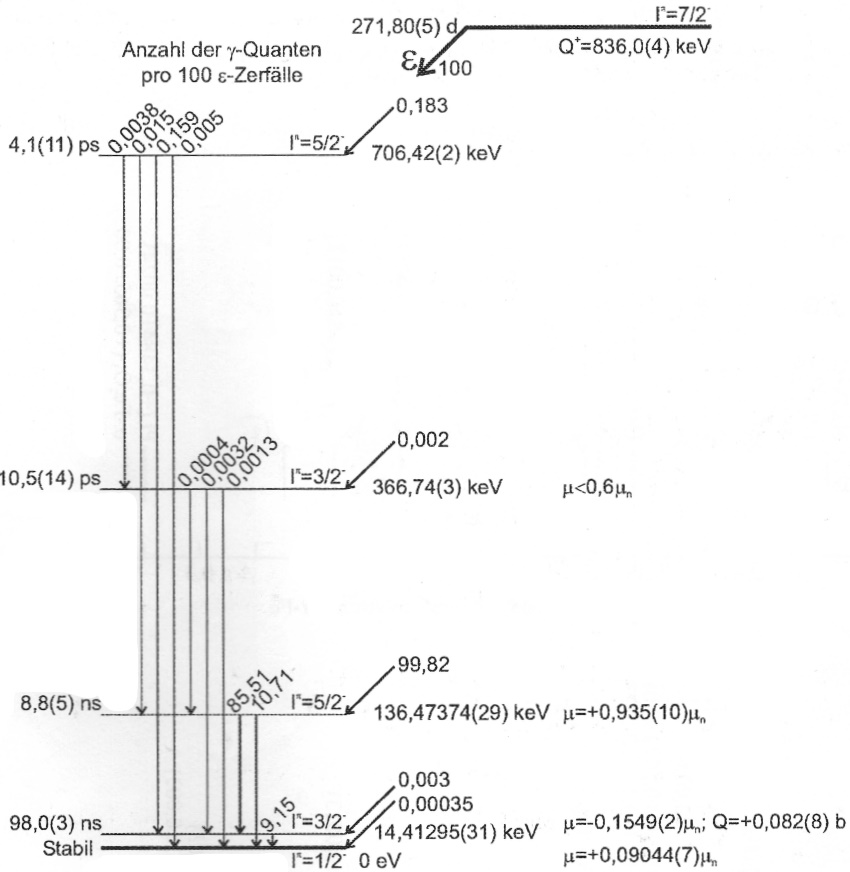
\includegraphics[width=0.9\linewidth]{img/Zerfallsschema}
		\caption{Zerfallsschema von $^{57}$Co.\cite{wwu}}
		\label{fig:zerfallsschema}
	\end{figure}
